\begin{figure}
    \centering
    \caption{Die SLIC-Pixelgrenzen sind in rot dargestellt }
    \label{fig:slic_parameters}
    \subfloat[ \(m = 0.1\)]{
        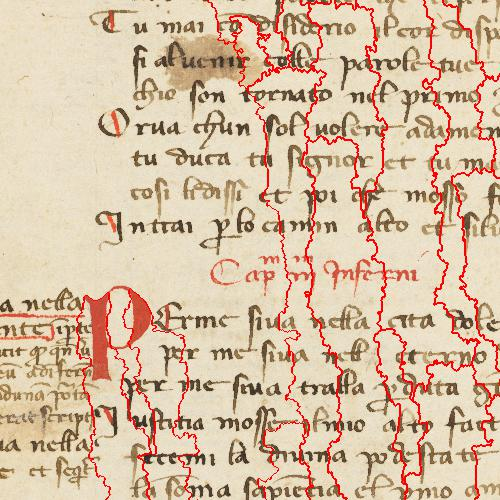
\includegraphics[width=0.24\textwidth]{figures/img/mark_boundaries_m0.jpg}
    }
    \subfloat[\(m = 1\)]{
        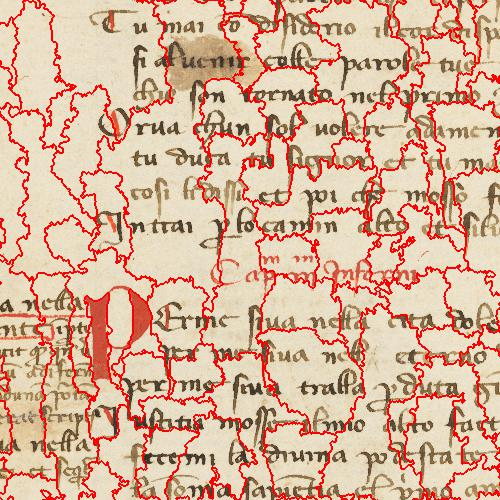
\includegraphics[width=0.24\textwidth]{figures/img/mark_boundaries_m1.jpg}
    }
    \subfloat[\(m = 10\)]{
        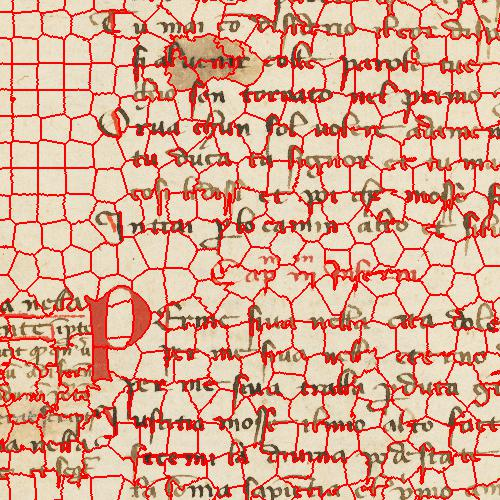
\includegraphics[width=0.24\textwidth]{figures/img/mark_boundaries_m10.jpg}
    }
    \subfloat[\(m = 100\)]{
        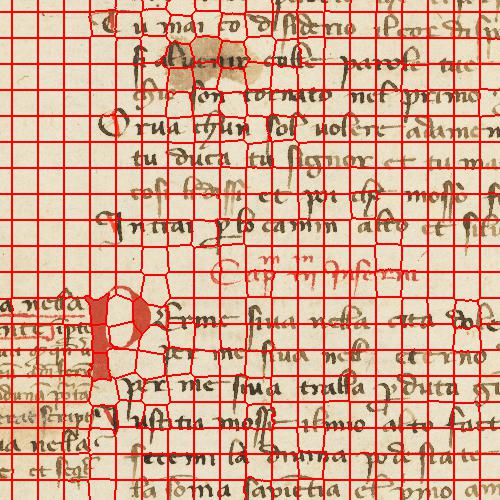
\includegraphics[width=0.24\textwidth]{figures/img/mark_boundaries_m100.jpg}
    }
\end{figure}